\documentclass[11pt]{article}
\usepackage{amsmath, amssymb, physics, mathtools, bm}
\usepackage{tikz, pgfplots}
\pgfplotsset{compat=1.18}
\usepackage[margin=2.3cm]{geometry}
\usepackage{siunitx, booktabs, hyperref}
\newcommand{\D}{\mathrm{D}}
\newcommand{\de}{\mathrm{d}}
\newcommand{\pd}[2]{\frac{\partial #1}{\partial #2}}
\newcommand{\pdd}[2]{\frac{\partial^{2} #1}{\partial #2^{2}}}
\newcommand{\Lap}{\nabla^{2}}
\title{B6 Condensed Matter Physics, 2025 --- Model Solutions}
\author{}
\date{}
\begin{document}
\maketitle

%======================================================================
\section*{Question 1 --- X-ray diffraction from CaF$_2$}

\textbf{Problem.} CaF$_2$ is fcc with Ca at $(0,0,0)$ and F at $\tfrac14(1,1,1)$, $\tfrac34(1,1,1)$. Define $S(\mathbf G)$, derive $S_{hkl}$, identify the first two strong powder lines at $2\theta=\ang{28.27},\ang{47.00}$ ($\lambda=\SI{0.15406}{nm}$), and estimate $I_{111}/I_{220}$.

\subsection*{(a) Definition and use of the structure factor}

Sum of basis scatterers, weighted by atomic form factor $f_j(\mathbf G)$ (Fourier transform of electron density, $f_j(0)=Z_j$):
\begin{equation}
S(\mathbf{G}) \;=\; \sum_{j \in \text{basis}} f_j(\mathbf{G})\, e^{\,i\mathbf{G}\cdot\mathbf{r}_j}.
\label{eq:Sdef}
\end{equation}
Kinematic (first Born) approximation: $I(\mathbf G)\propto\abs{S(\mathbf G)}^2$ (Lorentz/polarisation/multiplicity ignored). Reflections with $S=0$ are systematically absent.

For cubic $a$, $\mathbf G_{hkl}=(2\pi/a)(h,k,l)$. Laue $\mathbf k'-\mathbf k=\mathbf G$ for elastic scattering is equivalent to $\lambda=2 d_{hkl}\sin\theta$ with $d_{hkl}=2\pi/\abs{\mathbf G_{hkl}}$.

\subsection*{(b) Structure factor of CaF$_2$}

Fcc Bravais factor:
\begin{equation}
F_{\text{fcc}}(hkl) \;=\; 1 + e^{\,i\pi(h+k)} + e^{\,i\pi(k+l)} + e^{\,i\pi(h+l)},
\label{eq:Ffcc}
\end{equation}
which is $4$ for $h,k,l$ all-even or all-odd, else $0$. With basis at $(0,0,0)$ and $\tfrac14(1,1,1),\tfrac34(1,1,1)$, $\mathbf G\cdot\tfrac14(1,1,1)a=\tfrac\pi 2(h+k+l)$, so the basis sum is
\[
f_{\text{Ca}}+f_{\text{F}}\!\left[e^{i\pi(h+k+l)/2}+e^{i3\pi(h+k+l)/2}\right]=f_{\text{Ca}}+2f_{\text{F}}\cos\!\left[\tfrac\pi 2(h+k+l)\right].
\]
Hence
\begin{equation}
\boxed{\;S_{hkl} \;=\; F_{\text{fcc}}(hkl)\Big[\, f_{\text{Ca}} + 2 f_{\text{F}}\cos\!\big(\tfrac{\pi}{2}(h+k+l)\big)\,\Big]\;}
\label{eq:Scaf2}
\end{equation}
with $F_{\text{fcc}}=4$ on allowed reflections.

Three regimes: $h+k+l=4n$ gives $S\propto f_{\text{Ca}}+2f_{\text{F}}$ (strong); $h+k+l=4n+2$ gives $S\propto f_{\text{Ca}}-2f_{\text{F}}$ (near-extinct since $f_{\text{Ca}}\approx 2f_{\text{F}}$); $h+k+l$ odd gives $S\propto f_{\text{Ca}}$ (F ions cancel).

\subsection*{(c) Indexing the powder pattern and lattice constant}

$002$: $h+k+l=2$, so $S_{002}\propto f_{\text{Ca}}-2f_{\text{F}}\approx 0$ (near-extinct). $111$: $S_{111}\propto f_{\text{Ca}}$ (large).

Bragg + cubic:
\begin{equation}
\sin^2\theta \;=\; \frac{\lambda^2}{4 a^2}\,(h^2+k^2+l^2).
\label{eq:Bragg}
\end{equation}
$\theta_1=\ang{14.135}$, $\theta_2=\ang{23.50}$: $\sin^2\theta_1=0.05963$, $\sin^2\theta_2=0.15903$, ratio $2.667\approx 8/3$. Assign $111$ ($h^2+k^2+l^2=3$) and $220$ ($=8$); $200$ skipped (weak, same argument as $002$).

\[
a \;=\; \frac{\lambda \sqrt{3}}{2\sin\theta_{111}} \;=\; \frac{0.15406\times 1.7321}{2\times 0.24417}\,\si{nm}\;\approx\;\SI{0.5466}{nm}.
\]
Cross-check from $220$: $a\approx\SI{0.5464}{nm}$.
\begin{equation}
\boxed{\;\;\text{First two strong reflections: } 111 \text{ and } 220, \quad a \approx \SI{0.547}{nm}.\;\;}
\label{eq:abox}
\end{equation}

\subsection*{(d) Form-factor graphs and intensity ratio of 111 versus 220}

$f(G)$ is the Fourier transform of the ionic electron density: starts at $f(0)=Z_{\text{ion}}$ (here $f_{\text{Ca}^{2+}}(0)=18$, $f_{\text{F}^-}(0)=10$) and decays monotonically (closed shells).

At $a=\SI{5.466}{\angstrom}$:
\begin{equation}
G_{111}=\frac{2\pi\sqrt 3}{a}\approx \SI{1.99}{\angstrom^{-1}},\qquad G_{220}=\frac{2\pi\sqrt 8}{a}\approx \SI{3.25}{\angstrom^{-1}}.
\label{eq:Gnums}
\end{equation}
Reading off: $f_{\text{Ca}}(G_{111})\approx 14$, $f_{\text{F}}(G_{111})\approx 7$; $f_{\text{Ca}}(G_{220})\approx 11.5$, $f_{\text{F}}(G_{220})\approx 5.5$. Drop the common $F_{\text{fcc}}=4$:
\[
S_{111}=f_{\text{Ca}}+2f_{\text{F}}\cos(3\pi/2)=f_{\text{Ca}}\approx 14,\qquad S_{220}=f_{\text{Ca}}+2f_{\text{F}}\approx 22.5.
\]
\[
\frac{I_{111}}{I_{220}}=\frac{14^2}{22.5^2}\approx 0.39.
\]
\begin{equation}
\boxed{\;\; I_{111}/I_{220} \;\approx\; 0.4. \;\;}
\label{eq:Iratiobox}
\end{equation}
At 220 all three ions add coherently; at 111 the two F ions cancel and only Ca contributes.

%======================================================================
\section*{Question 2 --- 1D tight-binding model}

\textbf{Problem.} Chain of $N$ atoms, $\matrixel{n}{\hat H}{n}=\mathcal{E}_0$, $\matrixel{n}{\hat H}{n\pm 1}=-t$, PBC. (a) Find $E(k)$ and $g(E)$. (b) Half-filled (monovalent) molar $C$ and $\chi$; comment on divalent. (c) Add $\matrixel{n}{\hat H}{n\pm 2}=-t/2$; modified $E(k)$, $g(E)$.

\subsection*{(a) Band $E(k)$, bandwidth, and density of states}

Bloch ansatz $\ket k=N^{-1/2}\sum_n e^{ikna}\ket n$, PBC fixes $k=2\pi m/(Na)$, $N$ values in $(-\pi/a,\pi/a]$. Acting with $\hat H$:
\[
\hat H\ket k=\frac{1}{\sqrt N}\sum_n(\mathcal E_0-te^{-ika}-te^{ika})e^{ikna}\ket n=(\mathcal E_0-2t\cos ka)\ket k.
\]
\begin{equation}
\boxed{\;E(k) \;=\; \mathcal{E}_0 - 2t \cos ka, \qquad A = \mathcal{E}_0,\quad B = -2t.\;}
\label{eq:Ek}
\end{equation}
\begin{equation}
\boxed{\;W \;=\; 4t.\;}
\label{eq:bandwidth}
\end{equation}

DOS (factor 2 spin, factor 2 from $\pm k$, $k$-density $Na/2\pi$):
\[
g(E)=\frac{2Na}{\pi}\abs{\frac{\de k}{\de E}}=\frac{2Na}{\pi}\cdot\frac{1}{\abs{2ta\sin ka}}.
\]
Invert dispersion:
\[
\cos ka \;=\; \frac{\mathcal{E}_0 - E}{2t}.
\]
Apply $\sin^2 = 1 - \cos^2$:
\[
\sin^2 ka \;=\; 1 - \left(\frac{E-\mathcal{E}_0}{2t}\right)^{2}.
\]
Take positive root:
\[
\abs{\sin ka} \;=\; \sqrt{\,1 - \bigl[(E-\mathcal{E}_0)/(2t)\bigr]^{2}\,}.
\]
Substitute into denominator:
\[
\abs{2ta\sin ka} \;=\; 2ta\sqrt{\,1 - \bigl[(E-\mathcal{E}_0)/(2t)\bigr]^{2}\,}.
\]
Combine with prefactor $2Na/\pi$:
\begin{equation}
g(E) \;=\; \frac{N}{\pi t}\,\frac{1}{\sqrt{1-\bigl[(E-\mathcal{E}_0)/(2t)\bigr]^{2}}} \;=\; \frac{\alpha N}{\sqrt{1 - \beta(E-\mathcal{E}_0)^{2}}},
\label{eq:gE2}
\end{equation}
\begin{equation}
\boxed{\;\alpha = \frac{1}{\pi t},\qquad \beta = \frac{1}{4 t^{2}}.\;}
\label{eq:abox2}
\end{equation}
Integrable $1/\sqrt{}$ van Hove divergences at $E=\mathcal E_0\pm 2t$.

\begin{center}
\begin{tikzpicture}[>=stealth, scale=1.0]
  % Band E(k)
  \draw[->] (-3.8,0) -- (3.8,0) node[right] {$k$};
  \draw[->] (0,-2.0) -- (0,2.6) node[above] {$E(k)$};
  \draw[domain=-3.14:3.14, samples=120, thick]
    plot ({\x},{-1.5*cos(\x*180/3.14)});
  \draw[dashed] (-3.14,-1.5) -- (-3.14,1.7);
  \draw[dashed] ( 3.14,-1.5) -- ( 3.14,1.7);
  % High-symmetry points BELOW axis
  \node[below] at (-3.14,-0.05) {$-\pi/a$};
  \node[below] at ( 3.14,-0.05) {$\pi/a$};
  \node[below] at (0,-0.05) {$\Gamma$};
  % Critical points marked
  \node[circle,fill,inner sep=1.2pt,label=above right:{$\mathcal{E}_0+2t$}]
    at (3.14,1.5) {};
  \node[circle,fill,inner sep=1.2pt,label=below right:{$\mathcal{E}_0-2t$}]
    at (0,-1.5) {};

  % DOS panel
  \begin{scope}[xshift=9.0cm]
    \draw[->] (-0.3,0) -- (5.0,0) node[right] {$E$};
    \draw[->] (0,-0.3) -- (0,3.2) node[above] {$g(E)$};
    \draw[domain=0.06:3.94,samples=120,thick]
      plot ({\x},{0.5/sqrt(1-((\x-2)/2)^2)});
    % van Hove singularities
    \draw[dashed] (0,0) -- (0,2.8);
    \draw[dashed] (4,0) -- (4,2.8);
    \node[below] at (0,-0.05) {$\mathcal{E}_0-2t$};
    \node[below] at (4,-0.05) {$\mathcal{E}_0+2t$};
    \node[below] at (2,-0.05) {$\mathcal{E}_0$};
    \node[circle,fill,inner sep=1.2pt] at (2,0.5) {};
    \node[right] at (3.0,2.6) {van Hove};
  \end{scope}
\end{tikzpicture}
\end{center}

\subsection*{(b) Heat capacity and susceptibility for a half-filled band}

Monovalent: $N$ electrons in $2N$ states $\Rightarrow$ half-filled, $E_F=\mathcal E_0$. From \eqref{eq:gE2}, $g(E_F)=N/(\pi t)$.

Sommerfeld:
\[
C_V \;=\; \frac{\pi^2}{3}\,g(E_F)\,k_B^2\, T.
\]
Substitute $g(E_F)=N/(\pi t)$:
\[
C_V \;=\; \frac{\pi^2}{3}\,\frac{N}{\pi t}\,k_B^2\, T.
\]
Cancel $\pi$:
\[
C_V \;=\; \frac{\pi}{3}\,N k_B\,\frac{k_B T}{t}.
\]
Per mole ($N=N_A$):
\begin{equation}
C \;=\; \frac{\pi}{3}\,R\,\frac{k_B T}{t},\qquad
\boxed{\;\xi = 1, \qquad \eta = \pi/3.\;}
\label{eq:xibox}
\end{equation}

Pauli susceptibility:
\[
\chi_P=\mu_0\mu_B^2 g(E_F)/V.
\]
Per mole:
\begin{equation}
\boxed{\;\chi \;=\; \mu_0 \mu_B^{2}\,\frac{N_A}{\pi t}\;=\;\frac{\mu_0\mu_B^{2} R}{\pi t k_B}.\;}
\label{eq:chiPauli}
\end{equation}
Temperature-independent.

\emph{Divalent.} $2N$ electrons fill the band; $\mu$ in gap above. Insulator: $C_{\text{el}}\propto e^{-E_g/k_BT}$ (phonon $T^3$ dominates), $\chi_P\to 0$ (only small Landau/core diamagnetism).

\subsection*{(c) Adding second-neighbour hopping}

Second-neighbour adds $-(t/2)(e^{-2ika}+e^{2ika})=-t\cos 2ka$:
\begin{equation}
\boxed{\;E(k) \;=\; \mathcal{E}_0 - 2 t \cos ka - t \cos(2ka).\;}
\label{eq:Ek2}
\end{equation}
Extrema: $\de E/\de k=2ta\sin ka(1+2\cos ka)=0\Rightarrow ka=0,\pm 2\pi/3,\pm\pi/a$. Values: $E(0)=\mathcal E_0-3t$ (global min), $E(\pm 2\pi/3a)=\mathcal E_0+3t/2$ (global max), $E(\pm\pi/a)=\mathcal E_0+t$ (local min).

\begin{center}
\begin{tikzpicture}[>=stealth, scale=1.0]
  % Band with second-neighbour hopping
  \draw[->] (-3.8,-2.2) -- (3.8,-2.2) node[right] {$k$};
  \draw[->] (0,-3.4) -- (0,2.4) node[above] {$E(k)-\mathcal{E}_0$};
  \draw[domain=-3.14:3.14, samples=160, thick]
    plot ({\x},{-2*cos(\x*180/3.14) - cos(2*\x*180/3.14)});
  \draw[dashed] (-3.14,-2.2) -- (-3.14,1.0);
  \draw[dashed] ( 3.14,-2.2) -- ( 3.14,1.0);
  \draw[dashed] (-2.094,-2.2) -- (-2.094,1.5);
  \draw[dashed] ( 2.094,-2.2) -- ( 2.094,1.5);
  % High-symmetry k-points BELOW the axis
  \node[below] at (-3.14,-2.2) {$-\pi/a$};
  \node[below] at ( 3.14,-2.2) {$\pi/a$};
  \node[below] at (-2.094,-2.2) {$-2\pi/3a$};
  \node[below] at ( 2.094,-2.2) {$2\pi/3a$};
  \node[below] at (0,-2.2) {$\Gamma$};
  % Critical points
  \node[circle,fill,inner sep=1.2pt,label=below:{$-3t$}] at (0,-3) {};
  \node[circle,fill,inner sep=1.2pt,label=above right:{$+t$}] at (3.14,1) {};
  \node[circle,fill,inner sep=1.2pt,label=above:{$+3t/2$}] at (2.094,1.5) {};
  \node[circle,fill,inner sep=1.2pt] at (-3.14,1) {};
  \node[circle,fill,inner sep=1.2pt] at (-2.094,1.5) {};

  % DOS panel
  \begin{scope}[xshift=9.0cm]
    \draw[->] (-1.2,0) -- (5.2,0) node[right] {$E-\mathcal{E}_0$};
    \draw[->] (0,-0.3) -- (0,3.2) node[above] {$g(E)$};
    \draw[thick] (0,0.5) .. controls (0.5,0.4) and (1.0,0.5) .. (1.5,0.6);
    \draw[thick] (1.5,0.6) .. controls (2.0,0.8) and (2.4,1.5) .. (2.5,2.5);
    \draw[thick] (2.5,2.5) .. controls (2.7,2.5) and (3.0,1.4) .. (3.5,1.0);
    \draw[thick] (3.5,1.0) .. controls (4.0,0.7) and (4.4,2.5) .. (4.5,2.5);
    % van Hove singularities marked dashed and OUTSIDE the curve
    \draw[dashed] (0,0) -- (0,2.9);
    \draw[dashed] (2.5,0) -- (2.5,2.9);
    \draw[dashed] (4.5,0) -- (4.5,2.9);
    \node[below] at (0,-0.05) {$-3t$};
    \node[below] at (2.5,-0.05) {$+t$};
    \node[below] at (4.5,-0.05) {$+3t/2$};
    \node[circle,fill,inner sep=1.2pt] at (0,0.5) {};
    \node[circle,fill,inner sep=1.2pt] at (2.5,2.5) {};
    \node[circle,fill,inner sep=1.2pt] at (4.5,2.5) {};
  \end{scope}
\end{tikzpicture}
\end{center}
Three van Hove singularities, at $E=\mathcal E_0-3t,+t,+3t/2$.

%======================================================================
\section*{Question 3 --- Semiconductors and the Hall effect}

\textbf{Problem.} Define intrinsic/extrinsic semiconductors; derive $n(T)\propto T^\alpha e^{-\eta E_g/k_BT}$ and give $p(T)$. Define and measure $R_H$; use $R_H(300)/R_H(350)=28$ in undoped Si to get $E_g$. Estimate donor Bohr radius and ionisation energy in P-doped Si ($\epsilon_r=11.7$, $m^*=1.09\,m_e$); sketch $\ln R_H$ vs $1/T$.

\subsection*{(a) Intrinsic and extrinsic semiconductors}

\emph{Intrinsic}: pure host, valence full / conduction empty at $T=0$, gap $E_g$. Thermal pair excitation gives $n=p$. \emph{Extrinsic}: dopants put levels in the gap. Donors (e.g.\ P in Si) sit $E_d\ll E_g$ below $E_c$ and donate electrons; acceptors sit above $E_v$ and accept (creating holes). $n\neq p$ in general; majority carriers come from impurities.

\subsection*{(b) Conduction-band electron density $n(T)$}

Parabolic band:
\begin{equation}
g_c(E) \;=\; \frac{1}{2\pi^{2}}\!\left(\frac{2 m_e^{*}}{\hbar^{2}}\right)^{3/2}\sqrt{E - E_c}.
\label{eq:gc}
\end{equation}
Non-degenerate ($\mu$ in gap): use Maxwell--Boltzmann tail. With $x=(E-E_c)/k_BT$ and $\int_0^\infty\sqrt x e^{-x}\de x=\sqrt\pi/2$,
\begin{equation}
n(T) \;=\; N_c(T)\,e^{-(E_c-\mu)/k_B T},\qquad N_c(T) \;=\; 2\!\left(\frac{m_e^{*} k_B T}{2\pi\hbar^{2}}\right)^{3/2}.
\label{eq:nNc}
\end{equation}
Analogously for holes:
\begin{equation}
p(T) \;=\; N_v(T)\,e^{-(\mu-E_v)/k_B T},\qquad N_v(T)=2\!\left(\frac{m_h^{*} k_B T}{2\pi\hbar^{2}}\right)^{3/2}.
\label{eq:pNv}
\end{equation}
Mass action: $np=N_cN_v e^{-E_g/k_BT}\propto T^3 e^{-E_g/k_BT}$. Intrinsic neutrality $n=p$:
\[
n(T)=p(T)=\sqrt{N_cN_v}\,e^{-E_g/(2k_BT)}\propto T^{3/2}e^{-E_g/(2k_BT)}.
\]
\begin{equation}
\boxed{\;\alpha = 3/2, \qquad \eta = 1/2.\;}
\label{eq:nbox}
\end{equation}
\begin{equation}
\boxed{\;p(T) = n(T) \propto T^{3/2}\,e^{-E_g/(2 k_B T)}.\;}
\label{eq:pbox}
\end{equation}
The $E_g/2$ in the Boltzmann factor reflects $\mu$ pinned mid-gap.

\subsection*{(c) Hall coefficient: definition, measurement, and $E_g$ from undoped Si}

\emph{Definition.} With $j_x$, $B_z$, transverse field $E_y$ balances the Lorentz force in steady state:
\begin{equation}
R_H \;=\; \frac{E_y}{j_x B_z}.
\label{eq:RHdef}
\end{equation}
Single carrier of charge $q$, density $n$:
\begin{equation}
\boxed{\;R_H \;=\; \frac{1}{n q}.\;}
\label{eq:RHbox}
\end{equation}
Sign distinguishes electrons ($R_H<0$) from holes ($R_H>0$).

\emph{Measurement.} Thin rectangular bar; force longitudinal current $I$, measure transverse Hall voltage $V_H$ with high-impedance voltmeter. Width $w$, thickness $d$: $R_H=V_Hd/(IB)$. Reverse $B$ and average to remove offsets.

\emph{Why electrons dominate in Si.} $\mu_e\approx \SI{1400}{cm^2 V^{-1} s^{-1}}\gg\mu_h\approx \SI{450}{cm^2 V^{-1} s^{-1}}$; in two-carrier intrinsic Si, $R_H=(p\mu_h^2-n\mu_e^2)/[e(n\mu_e+p\mu_h)^2]<0$, electron-dominated.

\emph{Extracting $E_g$.} Use $R_H\propto 1/n$ with $n\propto T^{3/2}e^{-E_g/(2k_BT)}$:
\begin{equation}
\frac{R_H(300)}{R_H(350)} = \left(\frac{350}{300}\right)^{3/2}\!\exp\!\left[\frac{E_g}{2k_B}\!\left(\frac{1}{300}-\frac{1}{350}\right)\right]=28.
\label{eq:RHratio}
\end{equation}
Evaluate the prefactor:
\[
\left(\frac{350}{300}\right)^{3/2} \;\approx\; 1.260.
\]
Isolate the exponential:
\[
\exp\!\left[\frac{E_g}{2k_B}\!\left(\frac{1}{300}-\frac{1}{350}\right)\right] \;=\; \frac{28}{1.260} \;\approx\; 22.2.
\]
Take the logarithm:
\[
\frac{E_g}{2k_B}\!\left(\frac{1}{300}-\frac{1}{350}\right) \;=\; \ln 22.2 \;\approx\; 3.10.
\]
Evaluate the temperature factor:
\[
\frac{1}{300}-\frac{1}{350} \;=\; 4.762\times 10^{-4}\,\si{K^{-1}}.
\]
Solve for $E_g$:
\[
E_g \;=\; \frac{2k_B\times 3.10}{4.762\times 10^{-4}}\,\si{J} \;\approx\; 1.80\times 10^{-19}\,\si{J}.
\]
\begin{equation}
\boxed{\;E_g \;\approx\; \SI{1.12}{eV}.\;}
\label{eq:Egbox}
\end{equation}

\subsection*{(d) Donor Bohr radius and ionisation energy in P-doped Si}

Hydrogenic in dielectric medium with effective mass: $\epsilon_0\to\epsilon_0\epsilon_r$, $m_e\to m_e^*$:
\begin{equation}
a^{*} = \epsilon_r\frac{m_e}{m_e^{*}}a_0,\qquad E^{*}_R = \frac{1}{\epsilon_r^{2}}\frac{m_e^{*}}{m_e}E_R.
\label{eq:donscale}
\end{equation}
With $\epsilon_r=11.7$, $m_e^*/m_e=1.09$, $a_0=\SI{0.529}{\angstrom}$, $E_R=\SI{13.6}{eV}$, evaluate the Bohr radius:
\[
a^* \;=\; \frac{11.7}{1.09}\times 0.529\,\si{\angstrom} \;\approx\; \SI{5.68}{\angstrom}.
\]
Evaluate the Rydberg:
\[
E^*_R \;=\; \frac{1.09\times 13.6}{11.7^2}\,\si{eV} \;\approx\; \SI{0.108}{eV}.
\]
\begin{equation}
\boxed{\;a^{*} \approx \SI{0.57}{nm},\qquad E_d \approx \SI{0.11}{eV}.\;}
\label{eq:donbox}
\end{equation}
$a^*\gg a_{\text{Si}}$ justifies the dielectric continuum picture; experimental $E_d\approx \SI{45}{meV}$ for P:Si, the discrepancy from anisotropic mass and central-cell corrections.

\subsection*{(e) Sketch of $\ln R_H$ versus $1/T$ for the P-doped sample}

Three regimes (rising $T$):
\begin{enumerate}
\item Freeze-out ($k_BT\ll E_d$): $n\propto e^{-E_d/(2k_BT)}$, $\ln R_H$ rises with $1/T$, slope $\sim -E_d/2k_B$.
\item Saturation: all donors ionised, $n\approx N_d$, $\ln R_H$ flat.
\item Intrinsic: $n_i>N_d$, $\ln R_H\propto E_g/(2k_BT)$, steep slope $-E_g/2k_B$.
\end{enumerate}
Crossover when $\sqrt{N_cN_v}e^{-E_g/(2k_BT)}=N_d$; for $N_d=6.25\times 10^{18}\,\si{m^{-3}}$, $E_g=\SI{1.12}{eV}$, $T\sim \SI{500}{K}$.

\begin{center}
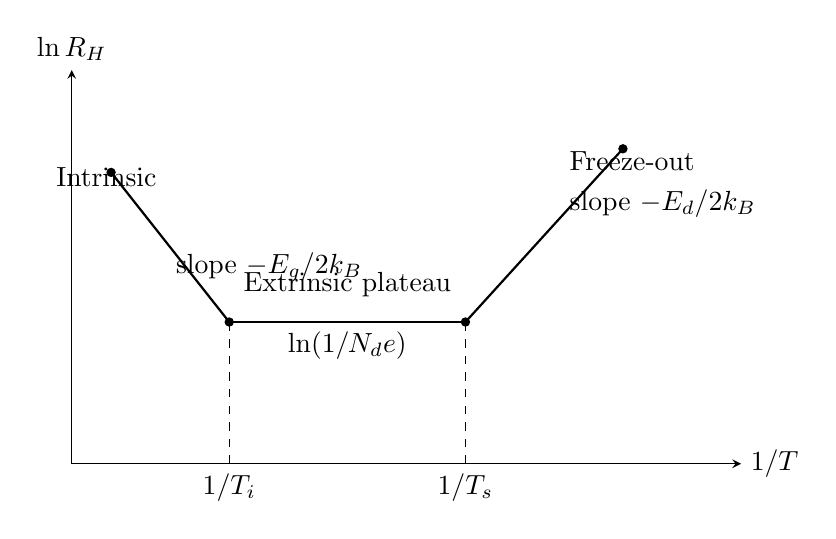
\begin{tikzpicture}[>=stealth, scale=1.0]
  \draw[->] (0,0) -- (8.5,0) node[right] {$1/T$};
  \draw[->] (0,0) -- (0,5.0) node[above] {$\ln R_H$};
  % Intrinsic (small 1/T, high T): steep
  \draw[thick] (0.5,3.7) -- (2.0,1.8);
  % Extrinsic plateau
  \draw[thick] (2.0,1.8) -- (5.0,1.8);
  % Freeze-out: steep again at large 1/T
  \draw[thick] (5.0,1.8) -- (7.0,4.0);
  % Markers at regime boundaries
  \node[circle,fill,inner sep=1.2pt] at (2.0,1.8) {};
  \node[circle,fill,inner sep=1.2pt] at (5.0,1.8) {};
  \node[circle,fill,inner sep=1.2pt] at (0.5,3.7) {};
  \node[circle,fill,inner sep=1.2pt] at (7.0,4.0) {};
  % Boundary tick marks BELOW axis
  \draw[dashed] (2.0,0) -- (2.0,1.8);
  \draw[dashed] (5.0,0) -- (5.0,1.8);
  \node[below] at (2.0,0) {$1/T_i$};
  \node[below] at (5.0,0) {$1/T_s$};
  % Region labels parked OUTSIDE the curve, well separated
  \node[above left] at (1.2,3.4) {Intrinsic};
  \node[below right] at (1.2,2.8) {slope $-E_g/2k_B$};
  \node[above] at (3.5,2.0) {Extrinsic plateau};
  \node[below] at (3.5,1.8) {$\ln(1/N_d e)$};
  \node[above right] at (6.2,3.6) {Freeze-out};
  \node[below right] at (6.2,3.6) {slope $-E_d/2k_B$};
\end{tikzpicture}
\end{center}

%======================================================================
\section*{Question 4 --- Heat capacity, Debye and magnetic contributions}

\textbf{Problem.} Compare Einstein/Debye assumptions; derive low-$T$ $C_{\text{Debye}}=xpR(T/T_D)^y$. For $N$ non-interacting $S=1/2$ spins derive $Z=[2\cosh z]^N$, hence $\chi$ and $C_{\text{mag}}$. Compare $C_{\text{mag}}/C_{\text{Debye}}$ at \SI{10}{K}, $B=\SI{0.1}{T}$ and $\SI{10}{T}$, with $T_D=\SI{200}{K}$, $p=10$, one magnetic atom per formula unit.

\subsection*{(a) Einstein versus Debye models}

Both: harmonic phonons, independent modes, Bose--Einstein occupation, Dulong--Petit limit $3Nk_B$ at high $T$.

Differ: Einstein gives all $3N$ modes $\omega=\omega_E$ (good for optical, zone-centre); $C\propto e^{-\hbar\omega_E/k_BT}$ at low $T$ --- too rapid. Debye uses linear acoustic dispersion $\omega=c_sk$ up to cutoff $\omega_D$ (mode count $=3N$); captures long-wavelength modes correctly, gives $C\propto T^3$.

\subsection*{(b) Debye internal energy and low-$T$ heat capacity}

Debye DOS (3 acoustic branches, $N_a$ atoms):
\begin{equation}
g(\omega) \;=\; \frac{9 N_a}{\omega_D^{3}}\,\omega^{2}, \qquad 0 \le \omega \le \omega_D.
\label{eq:gomegadebye}
\end{equation}
\[
U(T)=\int_0^{\omega_D}\de\omega\,g(\omega)\frac{\hbar\omega}{e^{\hbar\omega/k_BT}-1}.
\]
Substitute $x=\hbar\omega/k_BT$, $T_D=\hbar\omega_D/k_B$:
\[
U(T) \;=\; 9N_ak_BT\!\left(\frac{T}{T_D}\right)^3\!\!\int_0^{T_D/T}\!\!\frac{x^3\,\de x}{e^x-1}.
\]
Low $T$, extend the upper limit to $\infty$:
\[
U(T) \;\approx\; 9N_ak_BT\!\left(\frac{T}{T_D}\right)^3\!\!\int_0^{\infty}\!\!\frac{x^3\,\de x}{e^x-1}.
\]
Use $\int_0^\infty x^3/(e^x-1)\,\de x = \pi^4/15$:
\[
U(T) \;\approx\; 9N_ak_BT\!\left(\frac{T}{T_D}\right)^3\!\cdot\frac{\pi^4}{15}.
\]
Simplify:
\[
U(T) \;\approx\; \frac{3\pi^4}{5}\,N_ak_BT\!\left(\frac{T}{T_D}\right)^3.
\]
Differentiate with respect to $T$:
\[
C_V \;=\; \frac{12\pi^4}{5}\,N_ak_B\!\left(\frac{T}{T_D}\right)^3.
\]
Per mole of formula units, $N_a=pN_A$:
\begin{equation}
\boxed{\;C_{\text{Debye}}(T) \;=\; \frac{12\pi^{4}}{5}\, p R\!\left(\frac{T}{T_D}\right)^{3}, \qquad x = \frac{12\pi^{4}}{5},\; y = 3,\; T_D = \frac{\hbar\omega_D}{k_B}.\;}
\label{eq:CDbox}
\end{equation}

\subsection*{(c) Paramagnet: partition function, susceptibility, and $C_{\text{mag}}$}

$S=1/2$, $g_s=2$: $\epsilon_\pm=\mp\mu_B B$, so
\[
Z_1=2\cosh z,\qquad z\equiv\frac{\mu_B B}{k_B T}.
\]
Independent spins:
\begin{equation}
Z \;=\; [2\cosh(z)]^{N}.
\label{eq:Zspin}
\end{equation}

Free energy:
\[
F \;=\; -N k_B T\,\ln(2\cosh z).
\]
Magnetisation:
\[
M \;=\; -\frac{1}{V}\pd{F}{B} \;=\; \frac{N\mu_B}{V}\,\tanh z.
\]
Curie limit $z\ll 1$, expand $\tanh z \approx z$:
\[
M \;\approx\; \frac{N\mu_B}{V}\,z \;=\; \frac{N\mu_B^{2} B}{V k_B T}.
\]
Differentiate:
\begin{equation}
\chi(T) \;=\; \mu_0\,\pd{M}{B}\bigg|_{B=0} \;=\; \frac{\mu_0 N \mu_B^{2}}{V k_B T}.
\label{eq:chiCurie}
\end{equation}

Internal energy:
\[
U_{\text{mag}} \;=\; -N\mu_B B\,\tanh z.
\]
Use $\de z/\de T = -z/T$ and $\de(\tanh z)/\de z = \sech^2 z$:
\[
\frac{\de U_{\text{mag}}}{\de T} \;=\; -N\mu_B B\,\sech^2 z\cdot\left(-\frac{z}{T}\right).
\]
Simplify with $\mu_B B = z k_B T$:
\[
C_{\text{mag}} \;=\; N\mu_B B\,\sech^2 z\cdot\frac{z}{T} \;=\; N k_B\, z^2 \sech^2 z.
\]
Per mole of spins:
\begin{equation}
\boxed{\;C_{\text{mag}}(T,B) \;=\; R\,[f(z)]^{2}, \qquad f(z) = \frac{z}{\cosh z}, \qquad z = \frac{\mu_B B}{k_B T}.\;}
\label{eq:Cmagbox}
\end{equation}
Schottky form: $\propto z^2$ for $z\ll 1$, exponentially suppressed for $z\gg 1$, peak near $z\approx 1.2$.

\subsection*{(d) Numerical comparison and effect of strong interactions}

At $T=\SI{10}{K}$, evaluate the Debye prefactor:
\[
C_{\text{Debye}} \;=\; \frac{12\pi^4}{5}\cdot 10\cdot R\!\left(\frac{10}{200}\right)^3.
\]
Numerically:
\[
\frac{12\pi^4}{5}\cdot 10 \;\approx\; 233.78,\qquad \left(\frac{10}{200}\right)^3 \;=\; \frac{1}{8000}.
\]
Combine:
\[
C_{\text{Debye}} \;\approx\; \frac{233.78}{8000}\,R \;\approx\; 0.02923\,R.
\]
One mole of spins per mole of formula unit. With $\mu_B/k_B=\SI{0.6717}{K\,T^{-1}}$:

\textbf{(i) $B=\SI{0.1}{T}$:} evaluate $z$:
\[
z \;=\; \frac{\mu_B B}{k_B T} \;=\; \frac{0.6717\times 0.1}{10} \;\approx\; 6.72\times 10^{-3}.
\]
In the Curie limit $z\ll 1$:
\[
C_{\text{mag}} \;\approx\; R z^2 \;\approx\; 4.51\times 10^{-5}\,R.
\]
Ratio:
\begin{equation}
\boxed{\;\frac{C_{\text{mag}}}{C_{\text{Debye}}}\bigg|_{0.1\,\mathrm{T}} \;\approx\; 1.5\times 10^{-3}.\;}
\label{eq:rat1}
\end{equation}

\textbf{(ii) $B=\SI{10}{T}$:} evaluate $z$:
\[
z \;=\; \frac{0.6717\times 10}{10} \;=\; 0.6717.
\]
Evaluate $\cosh z$ and $f(z)=z/\cosh z$:
\[
\cosh z \;\approx\; 1.232,\qquad f(z) \;\approx\; \frac{0.6717}{1.232} \;\approx\; 0.5453.
\]
Hence:
\[
C_{\text{mag}} \;=\; R\,[f(z)]^2 \;\approx\; 0.2974\,R.
\]
\begin{equation}
\boxed{\;\frac{C_{\text{mag}}}{C_{\text{Debye}}}\bigg|_{10\,\mathrm{T}} \;\approx\; 10.\;}
\label{eq:rat2box}
\end{equation}
At \SI{10}{T} the Schottky term exceeds the phonon background by an order of magnitude --- the basis of adiabatic-demagnetisation cooling.

\emph{Strongly interacting spins at $B=0$.} Exchange $J$ generates an internal field; below $T_c\sim J/k_B$ the spins order. Expect:
\begin{itemize}
\item Lambda peak in $C_{\text{mag}}(T,0)$ at $T_c$ (second-order transition).
\item Magnon power law below $T_c$: $T^{3/2}$ (3D ferromagnet, $\omega\propto k^2$); $T^3$ (3D antiferromagnet, $\omega\propto k$).
\item High-$T$ tail $\propto 1/T^2$ from short-range correlations.
\item Total entropy $\int (C_{\text{mag}}/T)\de T=R\ln 2$ conserved (spin degeneracy).
\item Curie--Weiss susceptibility $\chi\propto 1/(T-\Theta_W)$, $\Theta_W\gtrless 0$ for FM/AFM.
\end{itemize}

\end{document}
